\section{\texorpdfstring{ASCII driver - Control Web}{ASCII driver - Control Web}}

% =====================================================================================================================
	\begin{frame}
    \frametitle{UART v PC}
    
    \begin{itemize}
      \item Moderní PC nemají port RS232 ani UART,
      \item v praxi se používají převodníky pro USB.
    \end{itemize}
    
    \vspace{3mm}
    
    \begin{minipage}[t][0.5\textheight][t]{0.48\textwidth}
      \textbf{USB-UART-TTL}
      
      \begin{center}
        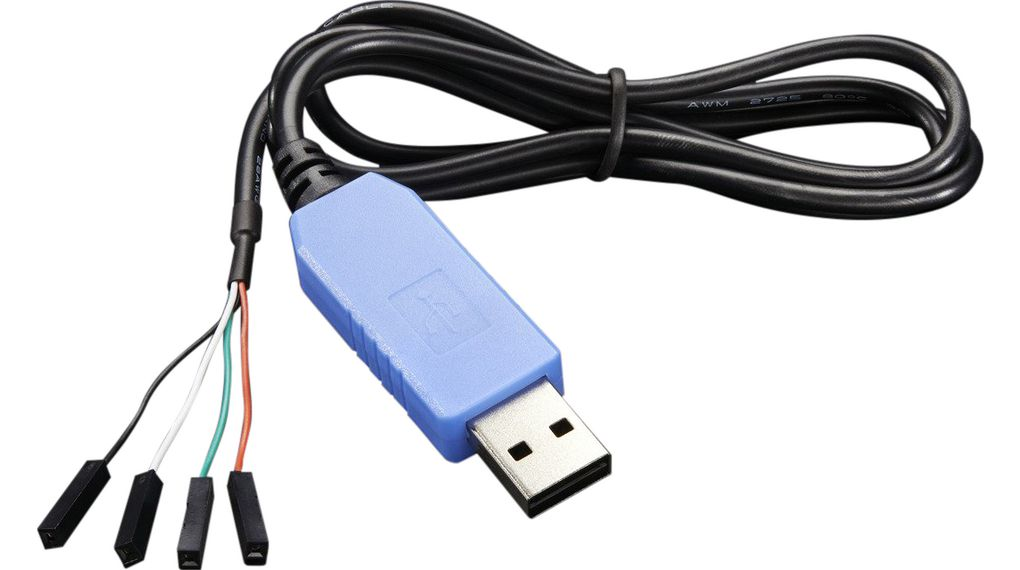
\includegraphics[width=1.00\textwidth]{fig/usb-uart.jpg}
      \end{center}
      
		\end{minipage}
		\begin{minipage}[t][0.5\textheight][t]{0.48\textwidth}
      \textbf{USB-RS232}
      
      \begin{center}
        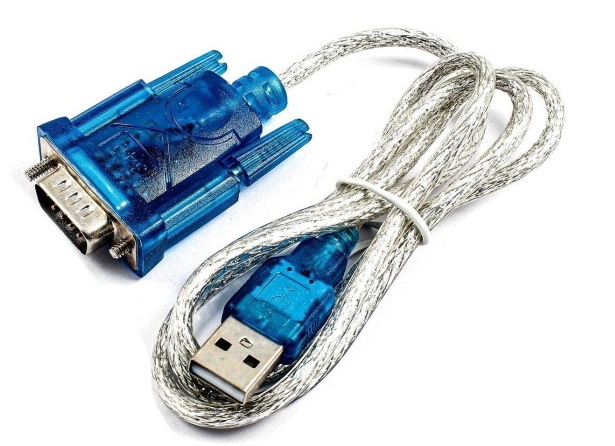
\includegraphics[width=1.00\textwidth]{fig/usb-rs232.jpg}
      \end{center}
      
		\end{minipage}
	\end{frame}
	
% =====================================================================================================================
	\begin{frame}
    \frametitle{Komunikace - požadavky}
    \small
		\begin{center}
			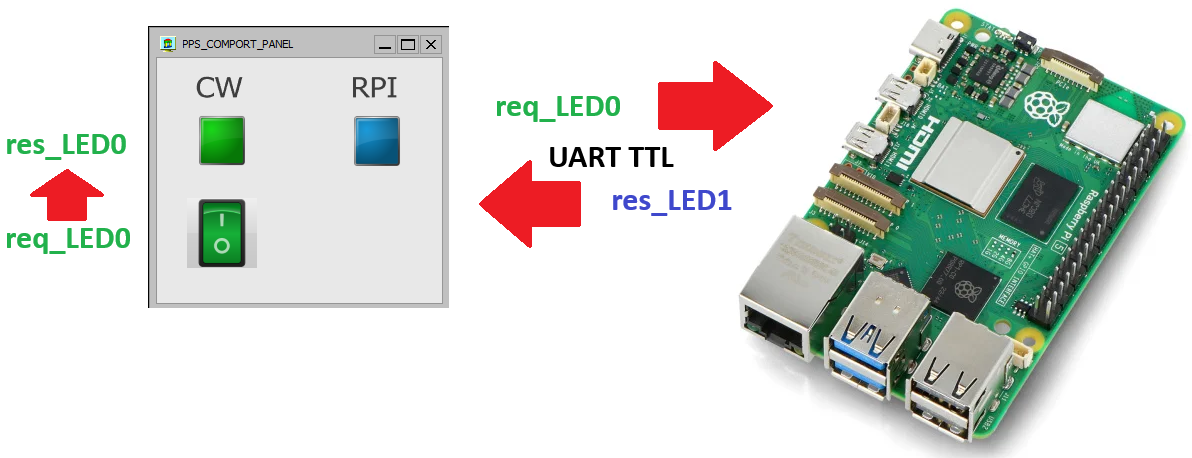
\includegraphics[width=1.00\textwidth]{fig/ascii_driver_variables.png}
		\end{center}
		
		\begin{itemize}
			\item Požadavek \textcolor{green}{\textbf{req\_LED0}} změní stav zelené led a zároveň je odeslán do RPI, které odpoví stejným stavem modré LED.
			\item \textbf{Nastavení sériové komunikace:} 115200 Bd, 8 bit, 1 stop bit, bez parity.
			\item \textbf{ASCII zprávy:} \uv{\textcolor{blue}{\textbf{LEDxH}}} pro log 1, \uv{\textcolor{blue}{\textbf{LEDxL}}} pro log 0.
		\end{itemize}
		
	\end{frame}
	
% =====================================================================================================================
	\begin{frame}
    \frametitle{Příprava proměnných a ovladače}

		\begin{center}
			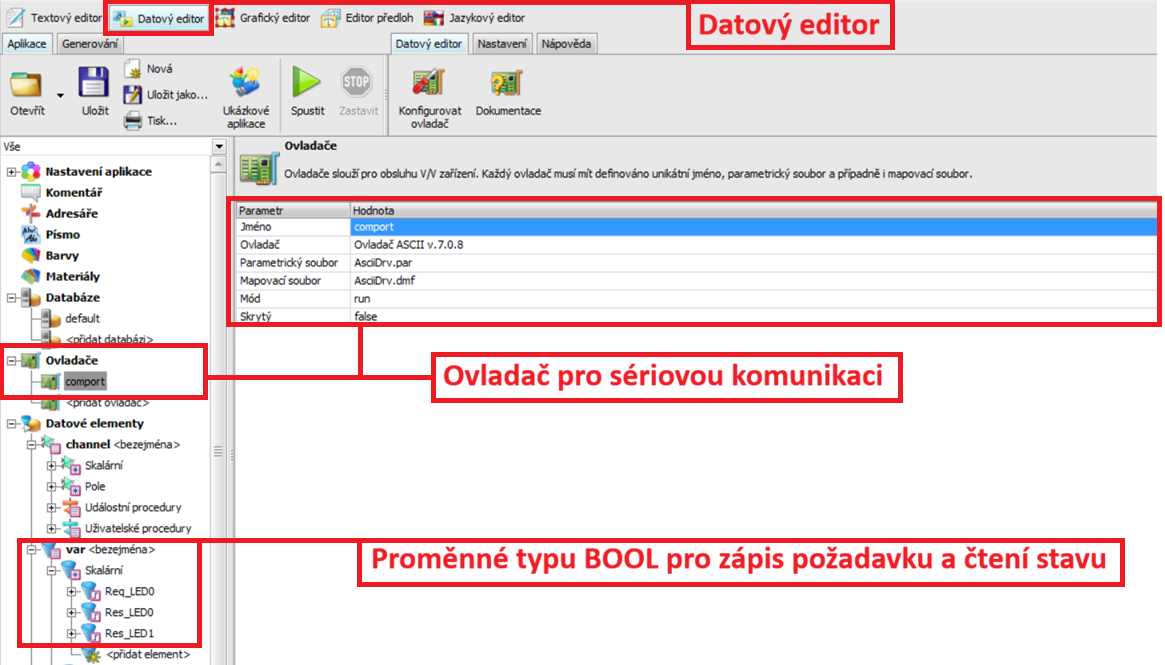
\includegraphics[width=1.00\textwidth]{fig/cw_driver.png}
		\end{center}
		
	\end{frame}
	
% =====================================================================================================================
	\begin{frame}
    \frametitle{Parametrický soubor ovladače}

		\begin{center}
			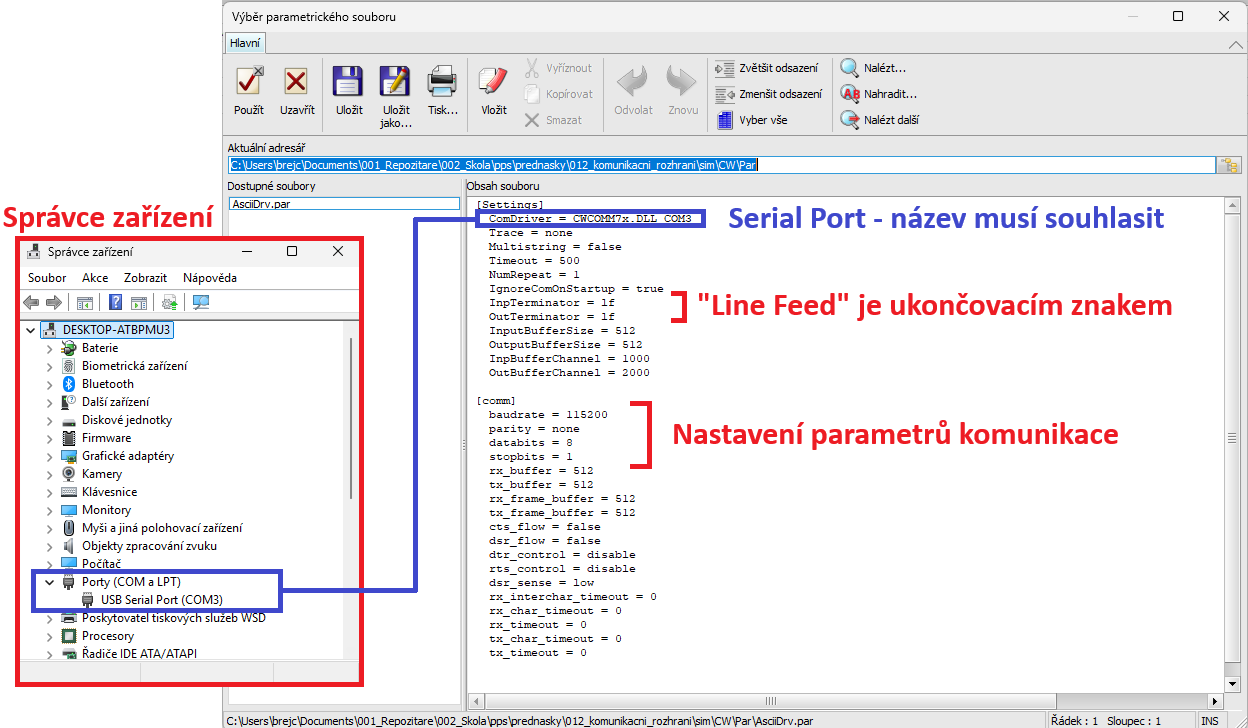
\includegraphics[width=1.00\textwidth]{fig/cw_driver_par.png}
		\end{center}
		
	\end{frame}
	
% =====================================================================================================================
	\begin{frame}
    \frametitle{Kanály ovladače}
		\small
		\begin{center}
			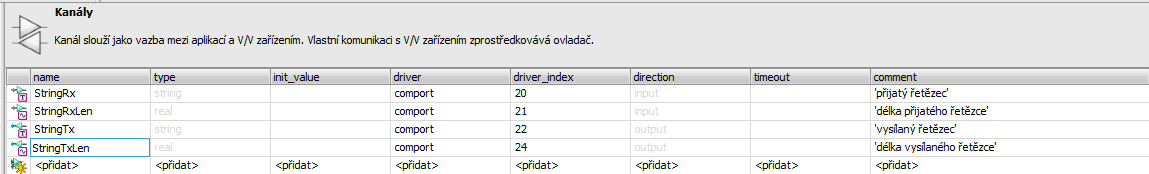
\includegraphics[width=1.00\textwidth]{fig/cw_driver_kanaly.png}
		\end{center}
		
		\vspace{3mm}
		Pro posílání a přijímání zpráv si vystačíme jen se dvěma kanály:
		
		\begin{itemize}
			\item \textbf{Kanál 22:} sem zapsaný řetězec se okamžitě vyšle po sériové lince, nečeká se na odpověď,
			\item \textbf{Kanál 23:} sem zapsaný řetězec se okamžitě vyšle po sériové lince, ale čeká se na odpověď,
			\item \textbf{Kanál 20:} reprezentuje poslední přijatý řetězec.
		\end{itemize}
		
		\vspace{3mm}
		Alternativně je možné používat přímá volání procedur ovladače předpisem:
		\begin{itemize}
			\item \textcolor{teal}{core}.DriverQueryProc(\textcolor{brown}{'driver'}, \textcolor{brown}{'procedura'}, \textcolor{blue}{hodnota})
		\end{itemize}
		
	\end{frame}
	
% =====================================================================================================================
	\begin{frame}
    \frametitle{Program}

		\begin{minipage}[t][\textheight][t]{0.48\textwidth}
      \textbf{ControlWeb}
      
			\begin{center}
				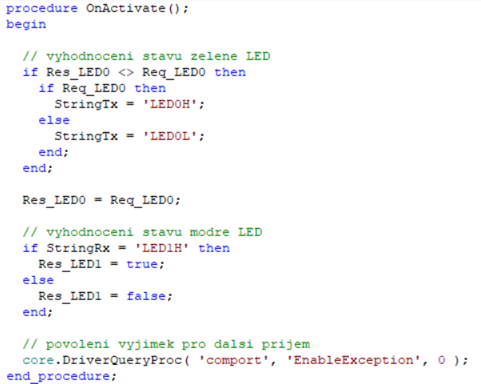
\includegraphics[width=1.00\textwidth]{fig/cw_driver_procedura.png}
			\end{center}
      
		\end{minipage}
		\begin{minipage}[t][\textheight][t]{0.48\textwidth}
      \textbf{RPI}
      
			\begin{center}
				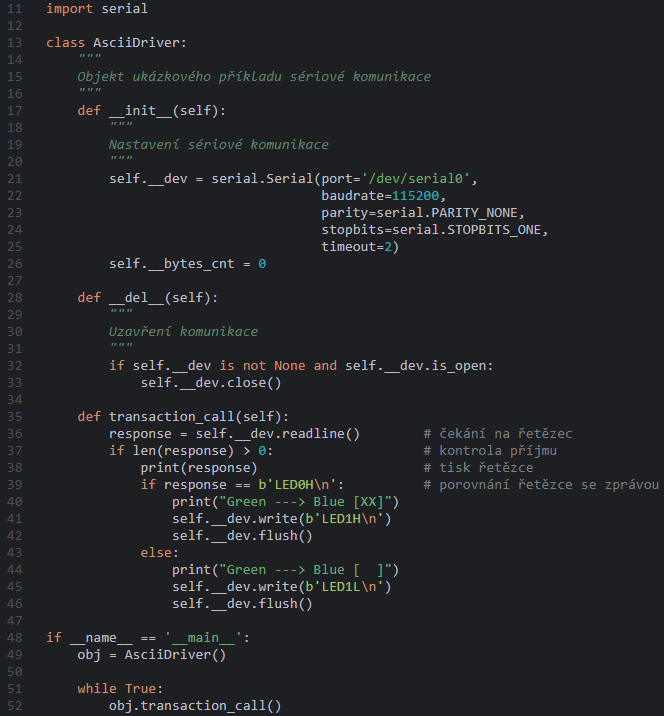
\includegraphics[width=1.00\textwidth]{fig/cw_driver_python.png}
			\end{center}
      
		\end{minipage}
		
	\end{frame}
	
% =====================================================================================================================
	\begin{frame}
    \frametitle{Logický analyzátor}

		\begin{center}
			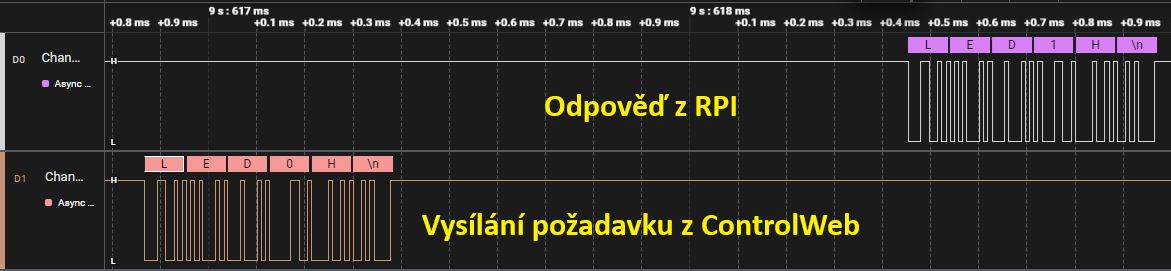
\includegraphics[width=1.00\textwidth]{fig/cw_driver_logan.png}
		\end{center}
		
		\vspace{3mm}
		
		\begin{itemize}
			\item Mezi příjmem požadavku a odpovědí je 1 ms zpoždění,
			\item každá zpráva trvá přibližně 500~$\mu$s,
			\item celkové minimální zpoždění reakce systému je kolem 2 ms,
			\item UART je jednoduché a snadno implementovatelné rozhraní, ale kvůli nižší přenosové rychlosti a režii rámců není vhodný pro velmi rychlé nebo časově kritické aplikace.
		\end{itemize}
		
	\end{frame}
	
% =====================================================================================================================
	\begin{frame}
    \frametitle{Srovnání UART a SPI}
		\small
		\begin{tabular}{|l|l|l|}
		\hline
		\textbf{Vlastnost} & \textbf{UART} & \textbf{SPI} \\ \hline
		Typ komunikace & asynchronní & synchronní \\ 
		Počet vodičů & 2 + GND & minimálně 4 \\ 
		Směr komunikace & full-duplex & full-duplex \\ 
		Topologie & bod--bod & master--slave \\ 
		Přenosová rychlost & nižší & velmi vysoká \\ 
		Režie přenosu & start/stop bity & minimální \\ 
		Adresace zařízení & ne & přes CS signály \\ 
		Více zařízení & komplikované & snadné \\ 
		Délka vedení & větší & spíše kratší \\ 
		Implementace & velmi jednoduchá & složitější \\ \hline
		Typické použití & terminály, SCADA, GPS & senzory, ADC, Flash \\ \hline
		\end{tabular}

		
	\end{frame}